\documentclass[12pt, letterpaper]{article}
\usepackage[hyphens]{url}
\setlength{\topmargin}{-1.75cm} \setlength{\textheight}{22.5cm}
\setlength{\oddsidemargin}{0.25cm}
\setlength{\evensidemargin}{0.25cm} \setlength{\textwidth}{16.2cm}
\renewcommand{\figurename}{Figure}
\usepackage{amssymb}
\usepackage{graphicx}
\usepackage{amsmath}
\usepackage{xcolor}
\usepackage[normalem]{ulem}
\usepackage{fontenc}
\usepackage{footnote}
\usepackage[breaklinks]{hyperref}
\usepackage{palatino, multicol, listings} % for multiple columns
\lstset{mathescape=true, basicstyle=\ttfamily,}

%\usepackage{pictex}
%% in the .pictex output of xfig, there is command \colo
%% however the old version of pictex may not define this
%% so we define color here as empty
%\def \color#1]#2{}

\begin{document}

\newcommand{\hide}[1]{}
\newcommand{\exercise}[1]{}
\newcommand{\future}[1]{}
\newcommand{\otherquestions}[1]{}
\newcommand{\set}[1]{\{#1\}}
\newcommand{\pg}[1]{{\tt #1}}
\newtheorem{definition}{Definition}
\newcommand{\emptyclause}{\Box}
\def\st{\bigskip\noindent}
\newcommand{\lplus}
{
   \stackrel{+}{\gets}
}

\newcommand{\fe}[1] {
  \begin{frame}
    #1
  \end{frame}}

\newcommand{\eoa}{ {\bf End} of algorithm}

\newcommand{\ft}[1] {\frametitle{#1}}

\newcommand{\ie}[1] {
  \begin{itemize}
    #1
  \end{itemize}
}

\newcommand{\ee}[1] {
  \begin{enumerate}
    #1
  \end{enumerate}\label{marker}
}
\newcommand{\blk}[2] {
  \begin{block}{#1}
    #2
  \end{block}
}

\newtheorem{collorary}{Corollary}
\newtheorem{proposition}{Proposition}
\newtheorem{invariant}{Invariant}
\newtheorem{property}{Property}
\newtheorem{claim}{Claim}
\newtheorem{example}{Example}


\title{P-log manual}
\date{\today}
\maketitle
\tableofcontents
\pagebreak


\section{System installation}

For the latest instructions on system installation, please refer to \url{https://github.com/iensen/plog2.0/wiki/Installation-Instructions}.
\section{System usage}\label{sysusage}

\medskip\noindent
The system requires programs to be stored in ASCII files.
The file can be of any extension (we recommend .pl or, not to be confused with Perl, .plog).

\medskip\noindent
A P-log file acceptable by the system should consist of:
\begin{enumerate}
\item P-log program, consisting of:
\begin{itemize}
\item sorts definitions,
\item attribute declarations, and
\item program rules.
\end{itemize}
\item Query.
\end{enumerate}

\st
For example, consider the following program:
\begin{verbatim}
sorts

#dice={d1,d2}.
#score={1,2,3,4,5,6}.
#person={mike,john}.
#bool = {true,false}.


attributes

roll:#dice->#score.
owns:#dice,#person->#bool.

statements

owns(d1,mike).
owns(d2,john).

random(roll(D)).

%probability information

pr(roll(D)=6|owns(D,mike))=1/4.

? roll(d1)=1.
\end{verbatim}


The program, originally introduced in \cite{gelfond2014knowledge}, describes a scenario with two dice being rolled, belonging to Mike and John respectively.
The second dice is more likely to produce \textit{6} as an outcome, as defined by the pr-atom
$$pr(roll(D)=6~|~owns(D,mike))=1/4.$$
By the so called \textit{principle of indifference} used by P-log, the probabilities of the remaining outcomes equal to (1 - 1/4)/5 = 3/20.
Thus, the answer to the query $roll(d1)=1$ is 1/8. Note that all outcomes of the second die are equally likely, so the answer to the query $roll(d2)=1$ is equal to 1/6.


\st
To compute the query probability using the system, we need to store it in a file and run the command:
$$plog2~[path\_to\_file]$$
where $plog2$ is the name of the p-log executable. For example, the file is stored in $plogapp/tests/paper/dice1.plog$ in our system, and we get the following output:

\begin{figure}[ht]
\centering
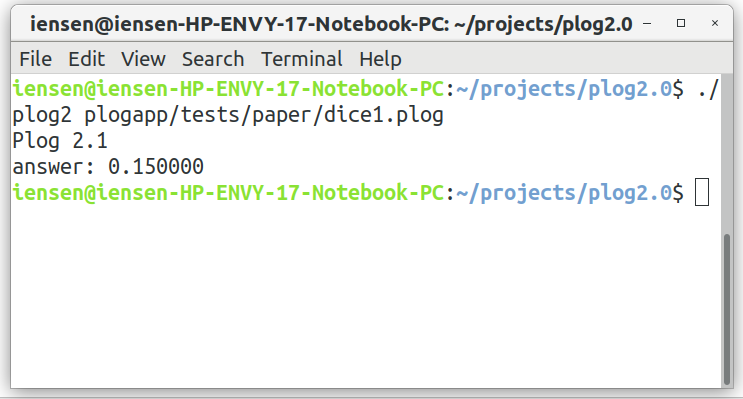
\includegraphics[width=0.9\textwidth]{plog_output.png}
\caption{P-log output}
\label{fig:plog_output}
\end{figure}


\st
The details of the syntax of the language can be found in \cite{Balai2019} and in the following sections. 

\section{Command Line Options}\label{option}

In this section we will describe the meanings of command line options supported by
P-log. As of right now, the system only accepts a single argument which is a path to the p-log file: 
\begin{itemize}
\item \textbf{input\_file} Specify the file where the sparc program is located.

\end{itemize}

\st
See Section \ref{sysusage} for an example of using this argument.


\section{Syntax Description}


\subsection{Sort definitions}\label{ss}


This section starts with a keyword $sorts$ followed by a collection of sort definitions of the form: 

\begin{equation*}
  sort\_name=sort\_expression.
\end{equation*}
\textit{sort\_name} is an identifier preceeded by the pound sign (\#).
\textit{sort\_expression}  on the right hand side denotes a collection of strings called $a~sort$.
\textcolor{red}{As of right now, the system only supports a basic sort definition of the form $sort\_name = \{t_1,\ldots,t_n\}$, where $t_1,\ldots,t_n$
  are ground terms. The remainder of the section is to be implemented in future.}.
  
\st
We divide all the sorts into \textit{basic sorts} and \textit{non-basic sorts}. 

\st \textit{Basic sorts} are defined as named collections of numbers and \textit{identifiers}, i.e, strings consisting of

\begin{itemize}

 \item letters: $\{a,b,c,d,...,z,A,B,C,D,...,Z\}$

 \item digits: $\{0,1,2,...,9\}$

 \item underscore: $\_$

\end{itemize}

and starting with a lowercase letter.



A \textit{non-basic sort} also contains at least one \textit{record} of the form $id(\alpha_1,\dots, \alpha_n)$ where $id$ is an identifier and 

$\alpha_1, \dots, \alpha_n$ are either identifiers, numbers or records. 



\st We define sorts by means of expressions (in what follows sometimes referred to as statements) of six types:
\begin{enumerate}


\item
\textbf{numeric range} is of the form:
\begin{equation*}
number_1..number_2
\end{equation*}
where $number_1$ and $number_2$ are non-negative numbers such that $number_1 \le number_2$. The expression defines the set 

of sequential numbers \\$\{number_1, number_1+1, \dots, number_2\}$.



\textit{Example:}



\begin{verbatim}

 #sort1=1..3.

\end{verbatim}

\texttt{\#sort1} consists of numbers $\{1,2,3\}$.


\item \textbf{identifier range} is of the form:

\begin{equation*}
  id_1..id_2
\end{equation*}

where $id_1$ and $id_2$ are identifiers both starting with a lowercase letter.

$id_1$ should be lexicographically \footnote{ The system default encoding is used for  ordering of individual characters} smaller than or equal to  $id_2$, and the length of $id_1$ must be less than or equal to the length of $id_2$. That is,  $id_1 \leq id_2$ and $|id_1| \leq |id_2|$.

The expression defines the set of strings  $\{s: id_1\leq s \leq id_2 \land |id_1|\leq |s| \leq |id_2|\}$.
\textit{Example:}

\begin{verbatim}
 #sort1=a..f.
\end{verbatim}

\texttt{\#sort1} consists of letters $\{a,b,c,d,e,f\}$.

\item \textbf{set of ground terms} is of the form:

\begin{equation*}
\{t_1,..,,t_n\}
\end{equation*}
The expression denotes a set of \textit{ground terms} $\{t_1,...,t_n\}$, defined as follows:
\begin{itemize}
 \item numbers and identifiers are ground terms;
 \item If $f$ is an identifier and $\alpha_1, \dots, \alpha_n$ are ground terms, 
then $f(\alpha_1,\dots, \alpha_n)$ is a ground term.
\end{itemize}

\textit{Example}: 
\begin{verbatim}
 #sort1={f(a),a,b,2}.
\end{verbatim}
\item \textbf{set of records} is of the form:

\begin{equation*}
f(sort\_name_1(var_1),..., sort\_name_n(var_n)):
                                     condition(var_1,...,var_n)
\end{equation*}
where $f$ is an identifier, for $ 1\leq i\leq m$ $sort\_name_i$ occurs in one of the preceeding sort definitions and  the condition on variables $var_1,...,var_n$ (written as $condition(var_1,...,var_n)$) is defined as follows:

\begin{itemize}
\item if $var_i$ and $var_j$ occur in the sequence  $var_1,...,var_n$ and $\odot$ is an element of $\{>,<,\le,\ge\}$, then $var_i \odot var_j$ is a condition on   $var_1,...,var_n$.
\item if $\mathcal{C}_1$ and $\mathcal{C}_2$ are both conditions on  $var_1,...,var_n$, and $\oplus$ is an element of  $\{\cup,\cap\}$, then
$(\mathcal{C}_1 \oplus \mathcal{C}_2)$ is a condition on  $var_1,...,var_n$.
\item if $\mathcal{C}$ is a  condition on  $var_1,...,var_n$, then $not(\mathcal{C})$ is also a condition on  $var_1,...,var_n$.
\end{itemize}
Variables $var_1,...,var_n$ occurring in parenthesis after sort names are optional as well as the condition :$condition(var_1,...,var_n)$.

If a condition contains a subcondition $var_i~\odot~var_j$,  then the sorts  $sortname_i$ and  $sortname_j$

must be defined by basic statements (the definition of a basic statement is given below after the definition of a concatenation statement).

The expression defines a collection of ground terms 
\\ $\{f(t_1,\dots,t_n):  t_1 \in s_i \land \dots \land t_n \in s_n \land (condition(X_1,\dots, X_n)|_{X_1 = t_1,\dots,X_n = t_n})\}$

\textit{Example}
\begin{verbatim}
 #s=1..2.
 #sf=f(s(X),s(Y),s(Z)): (X=Y or Y=Z). 
\end{verbatim}

The sort \texttt{\#sf} consists of records $\{f(1,1,2),f(1,1,1),f(2,1,1)\}$



 \item \textbf{set-theoretic expression} can be in one of the following forms:
\begin{itemize}
\item $\#sort\_name$  
\item an expression of the form (3), denoting a set of ground terms
\item an expression of the form (4), denoting a set of records
\item $(S_1 \bigtriangledown S_2)$, where $\bigtriangledown \in \{+,-,*\}$ and both $S_1$ and $S_2$ are set theoretic expressions
\end{itemize}

$\#sort\_name$ must be a name of a sort occurring in one of the preceeding sort definitions. 
The operations $+$ $*$ and $-$ stand for union, intersection and difference correspondingly.


\textit{Example} : 
\begin{verbatim}
 #sort1={a,b,2}.
 #sort2={1,2,3} + {a,b,f(c)} + f(#sort1).
\end{verbatim}
 \texttt{\#sort2} consists of ground terms $\{1,2,3,a,b,f(c),f(a),f(b),f(2)\}$.
\item \textbf{concatenation} is of the form
\begin{equation*}
 [b\_stmt_1] ... [b\_stmt_n]
\end{equation*}

$b\_stmt_1, \dots, b\_stmt_n$ must be \textit{basic statements}, defined as follows:


\begin{itemize}
 \item statements of the forms (1)-(3) are basic
 \item statement $S$ of the form (5) is basic if:
 \begin{itemize}
 \item it does not contain sort expressions of the form (4), denoting sets of records
  \item none of curly brackets occurring in $S$ contains a record
  \item all sorts occurring in $S$ are defined by basic statements 
 \end{itemize}
\end{itemize}
Note that basic statement can only define a basic sort.

\textit{Example\footnote{We allow a shorthand `b` for singleton  set \{b\}}.:}

\begin{verbatim}
 #sort1=[b][1..100].
\end{verbatim}

\texttt{sort1} consists of identifiers $\{b1,b2,\dots, b100\}$.

\end{enumerate}
\subsection{Attribute Declarations}

\noindent  The second part of a  P-log program starts with the keyword
\st
$attributes$

\st and is followed by statements of the form

\begin{equation*}
attr\_symbol : \#sortName_1,\dots,\#sortName_n \rightarrow \#sortName  
\end{equation*}
where $attr\_symbol$ is an identifier (in what follows referred to as an attribute symbol) and
$\#sortName$, $\#sortName_1$,\dots,$\#sortName_n$ are sorts defined in sort definitions section of the program.



Multiple declarations containing the same attribute symbol are not allowed.
Attributes with no arguments must be declared as $attr\_symbol:sortName_1$ (example: \texttt{a:\#bool}).

% \st For any sort name $\#s$, the system includes declaration  $\#s:\#s -> #boolean$ automatically. 

\subsection{Program Statements}

\st The third part of a P-log program starts with the keyword \textit{statements} followed by a collection \textit{rules} and \textit{pr-atoms} (in any order). Here we give a brief overview of the system assuming that a reader is familiar with notions of a term and a literal. For the details, please refer to \cite{Balai2019}. 

\subsubsection{Program Rules}
P-log rules are of the following form:

\begin{equation}
   a(t) = y \leftarrow l_1,  \ldots, l_k, not~l_{k+1} \ldots not~l_{n}.
 \end{equation}
where $a(t) = y$ is a program atom and $l_1,\ldots,l_k$ are program literals.
The atom $a(t) = y$ is referred to as the \textit{head} of the rule, and $l_1,\ldots,l_k$ is referred to as the \textit{body} of the rule.
 A rule with $k=0$ is referred to as a \textit{fact}.
 The system allows for a shorthand $a(t)$ for $a(t) = true$, and standard arithmetic relations of the form $t_1~op~t_2$, where $op \in \{\texttt{>=},\texttt{<=},\texttt{>},\texttt{<},\texttt{=},\texttt{!=}\}$ in the body of the rule .
 Three special kinds of rules are \textit{random selection rules}, \textit{observations} and \textit{actions}.
 As described in \cite{Balai2019},
 random selection rule is a rule whose head is of one of the forms $random(a,p)$ or $random(a)$. Action is a fact whose head is $do(a,y)$\footnote{The system doesn't support rule labels and actions of the form $do(r,a,y)$ described in \cite{Balai2019}. Therefore there has to be at most one action of each attribute term. This is a limitation we plan to overcome in future.}.
 Observation is a fact whose head is of the form $obs(a,y,t)$.

 \subsubsection{Pr-Atoms}

 Probability atoms (in short, pr-atoms) are of the form 
 $$pr(a(t) = y | B) = v.$$
 where $a(t) = y$ is a program atom, $B$ is a collection of e-literals and $v$  written as a fraction of the form $n/m$, where $n$ and $m$ are natural numbers.  Example:
\begin{center}
 \texttt{pr(roll(D)=6 | not owns(D,mike))=1/4.}
\end{center}
 \subsection{Program Examples}

 For a collection of working P-log programs used for system testing and development, please refer to
 \begin{center}
\url{https://github.com/iensen/plog2.0/tree/master/plogapp/tests}.
 \end{center}
 

 \section{Error Checking}

 \textcolor{red}{Please be aware that some of the errors are not implemented yet.}

\st
Additional error checking is performed when no syntax error is found. Majority of the errors are related to types.
\subsection{Type errors}
Type errors are considered as serious issues which make it  impossible to compile and execute the program.
Type errors can occur in all four sections of a P-log program.
\subsubsection{Sort definition errors}
The following are possible causes of a sort definition error  that will result in a type error  message from ${\cal SPARC}$:
\begin{enumerate}
\item  A set-theoretic expression (statement 5 in section \ref{ss}) containing a sort name that has not been defined.

\textit{Example:}
\begin{verbatim}
 sorts
 #s={a}.
 #s2=#s1-#s.
\end{verbatim}

\item  Declaring a sort more than once.

\textit{Example:}
\begin{verbatim}
 sorts
 #s={a}.
 #s={b}.
\end{verbatim}

\item An identifier range $id_1..id_2$ (statement 2 in section \ref{ss}) where $id_1$ is greater than $id_2$.

\textit{Example:}
\begin{verbatim}
 sorts
 #s=zbc..cbz.
\end{verbatim}

\item A numeric range $n_1..n_2$ (statement 1 in section \ref{ss}) where  $n_1$ is greater than $n_2$.

\textit{Example:}
\begin{verbatim}
 sorts
 #s=100500..1.
\end{verbatim}


\item A numeric range (statement 2 in section \ref{ss}) $n_1..n_2$ that  contains an undefined constant.

\textit{Example:}
\begin{verbatim}
 #const n1=5.
 sorts
 #s=n1..n2.
\end{verbatim}

\item An identifier range $id_1..id_2$ (statement 3 in section \ref{ss}) where  the length of $id_1$ is greater than the length of $id_2$. 


\textit{Example:}
\begin{verbatim}
 sorts
 #s=abc..a.
\end{verbatim}

\item A concatenation (statement  4 in section \ref{ss}) that contains a non-basic sort.

\textit{Example:}
\begin{verbatim}
 sorts
 #s={f(a)}.
 #sc=[a][#s].
\end{verbatim}



\item A record definition (statement 5 in section \ref{ss}) that contains an undefined sort.

\textit{Example:}
\begin{verbatim}
 sorts
 #s=1..2.
 #fs=f(s,s2).
\end{verbatim}



\item A record definition  (statement 5 in section \ref{ss}) that contains a condition with relation $>,<,\geq,\leq$ such that the
   corresponding sorts are not basic.

\textit{Example:}
\begin{verbatim}
#s={a,b}.
#s1=f(#s). 
#s2=g(s1(X),s2(Y)):X>Y.
\end{verbatim}

\item  A variable that is used more than once in a record definition (statement  5 in section \ref{ss}).

\textit{Example:}

\begin{verbatim}
 sorts
 #s1={a}.
 #s=f(#s1(X),#s1(X)):(X!=X).
\end{verbatim}
\item A sort that contains an empty collection of ground terms.

\textit{Example}
\begin{verbatim}
 sorts
 #s1={a,b,c}
 #s=#s1-{a,b,c}.
\end{verbatim}
\end{enumerate}
\subsubsection{Attribute declarations errors}

\begin{enumerate}
\item An attribute with the same name is defined more than once.
\textit{Example:}
\begin{verbatim}
 sorts
 #s={a}.
 attributes
 a: #s -> #s.
 a: #s,#s ->#s.
\end{verbatim}
\item An attribute declaration contains an undefined sort.
\textit{Example:}
\begin{verbatim}
 sorts
 #s={a}.
 attributes
 p:#ss.
\end{verbatim}
\end{enumerate}
\subsubsection{Program statements errors}

In program rules and pr-atoms we first check each atom of the form $a(t_1,\dots,t_n) = y$ and each term occurring in the program $\Pi$ for satisfying
the definitions of program atom and program term correspondingly (see Section 3 of \cite{Balai2019}).In addition, we check that no sort occurs in a head of a rule of $\Pi$.
\subsection{Type warnings}\label{type_warnings}
\textcolor{red}{This section is to be completed and implemented. At the very least, we plan to support finite-domain constraint-based typechecking which will flag rules with no ground instances.}

\bibliography{mybib}
\bibliographystyle{plain}
\end{document}


%%% Local Variables:
%%% mode: latex
%%% TeX-master: t
%%% End:
